\documentclass[letterpaper]{article}
\usepackage{uai2019}
\usepackage[margin=1in]{geometry}

% Set the typeface to Times Roman
\usepackage{times}
\usepackage[utf8]{inputenc}
\usepackage{mathtools}
\usepackage{amsfonts}
\usepackage{booktabs}
\usepackage{algorithm}
\usepackage{algpseudocode}
\usepackage[colorlinks=true,citecolor=blue,urlcolor=blue]{hyperref}

\newcommand{\mean}[1]{\left\langle #1 \right\rangle}
\newcommand{\avg}[1]{\langle#1\rangle}
\newcommand{\et}{\;\mathrm{and}\;}
\newcommand{\Real}{\mathbb{R}}
\newcommand{\STAB}{\mathrm{STAB}}
\renewcommand{\TH}{\mathrm{TH}}
\newcommand{\chull}{\mathrm{Conv}}
\DeclareMathOperator*{\PA}{PA}
\begin{document}
\title{Supplemental Materials}
\maketitle
\section*{Building the exclusivity graph from DAG}
In the following we describe in more details how to get from the DAG
(Directed Acyclic Graph) representation of a causal model to the one
for exclusivity graph.
Starting from a generic causal model described by a DAG $D$, with
$N$ random variables $O_D = \{A_1,\ldots,A_N\}$ and $M$ instruments
$I_D = \{X_1,\ldots,X_M\}$, the exclusivity graph $G = (V, E)$ can be
constructed, for example, using a simple breadth-first graph exploring
algorithm.
The procedure, described in algorithm \ref{alg:bfgb}, requires the DAG $D$
and the list $V$ of vertices to be explored, since we can be interested
in building the graph only for a subset of events.

\begin{algorithm*}
\caption{Breadth-first graph exploration}
\label{alg:bfgb}
\begin{algorithmic}[1]
\Function{build graph}{$V, D$} 
\State $E \gets \emptyset$
\While{$V \neq \emptyset$}
    \State $\Call{insert}{Q, V_1}$ \Comment{Initialize the queue with the first element of $V$}
    \State $\Call{delete}{V, V_1}$
    \While{$Q \neq \emptyset$}
        \State $v \gets Q_1$ 
        \State $\Call{delete}{Q, Q_1}$
        \For{$u \in V$}
            \If{\Call{exclusive}{$u$, $v$}}
                \State \Call{insert}{$E, (v, u)$}
                \State \Call{insert}{$Q, u$}
                \State \Call{delete}{$V, u$} \Comment{Visited nodes are removed from $V$}
        \EndIf
        \EndFor
    \EndWhile
\EndWhile
\State \Return E
\EndFunction
\end{algorithmic}
\vspace{1em}
As in the main text, here $a, a'$ stand for the value of the outcome of the
variable $A$ in the events $v, v'$, while $p_a, p_{a'}$ stand for the values
of the parent nodes of $A$ in $D$, $\PA (A)$.

\begin{algorithmic}[1]
\Function{exclusive}{$v, v', D$} 
    \State $n \gets \text{true}$
    \For{$A \in O_D$} 
        \State $n \gets n \land \left(p_a \neq p_{a'} \lor (p_a = p_{a'} \land a = a') \right)$
    \EndFor
    \State \Return $\neg n$
\EndFunction
\end{algorithmic}
\end{algorithm*}

\section*{Edge colored multigraph technique for approximating the quantum
bound}
\begin{figure}[t]
    \centering
    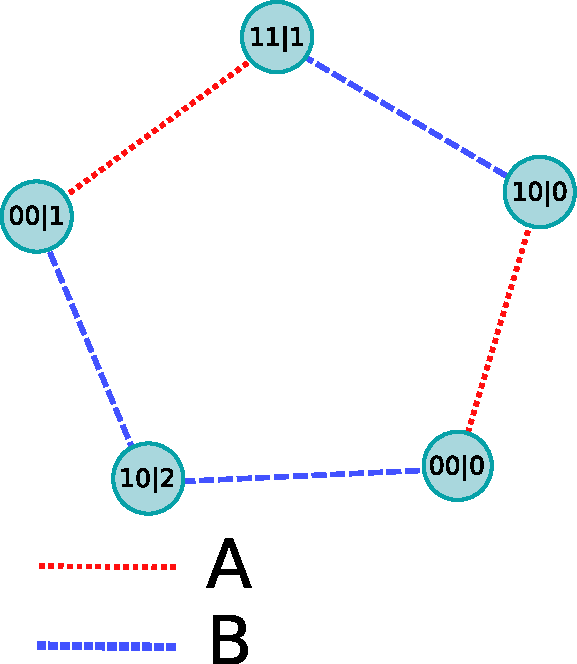
\includegraphics[width=.7\columnwidth]{images/instrumental_multigraph.pdf}
    \caption{Edge colored exclusivity graph representation of the Bonet
        inequality. Exclusivity constraints for the party $A$ and $B$ are
    represented by red lines and blue lines respectively.}
    \label{fig:instrumental_multigraph}
\end{figure}

The Lov\'asz theta of a graph, despite being efficiently computable,
only gives an upper bound to the maximal quantum bound, since it ignores
the additional constraints arising from the presence of different random
variables $A_i$.
Indeed the quantum bound is influenced not only by the exclusivity relations between the
possible events in our scenario, but also on how those relations are derived from the
variables $A_1,\ldots,A_N$.

To obtain a better approximation for the quantum bound we can follow
the technique presented in \cite{rabelo2014}.
This method consists in introducing an edge coloring in the exclusivity graph. 
This edge coloring encodes the information of which of the $A_i$s is involved in the exclusivity constraints under consideration.
In practice this corresponds to constructing an exclusivity graph $G_i$ for each
$A_i$. The resulting object is called a \emph{multigraph}. 
Having defined a multigraph $G = {G_1, \ldots, G_N}$ for a given scenario the
quantum bound is defined by the quantity:
\begin{equation}
    \vartheta(G) = \max_{v} \sum_{i \in V} |v \cdot a^1_i \otimes \dots \otimes a^n_i|^2
    \label{eq:multigraph_lovazs}
\end{equation}
where $\{a^j_i\}$ is an orthonormal labelling for $G_j$ and $V$ is the set
of vertices of $G$. This quantity, which can be seen as a generalization
of the Lov\'asz theta, is in general not efficiently computable, but,
as described in \cite{rabelo2014}, can be arbitrarily approximated by
a hierarchy of semi-definite programs\cite{npa2008}.

For example, in the case of the pentagon in the instrumental scenario we have two colors, and thus two graph $G_A$ and $G_B$, corresponding to variables $A$ and $B$ respectively, as shown in Fig.~\ref{fig:instrumental_multigraph}.
Applying the technique described above to this scenario yields a quantum
bound of $2.2071$, reproducing the known value for the quantum bound of the Bonet inequality given by $(3+\sqrt{2})/2$.

\section*{There are no quantum violation for instrumental scenarios with $l=2$
settings.}
It is easy to see that no quantum violation is possible for instrumental scenario
with $l=2$ possible settings for the instrumental variable $X$.
This reduces to proving that there are no odd $n$-cycles nor $n$-anticycles as induced
subgraphs in the corresponding exclusivity graph, with $n\ge5$.
To see this we can notice that any such graph is composed by two cliques (see
for example Fig.~\ref{fig:2mn_nocycle_proof}), corresponding to the events with $x=0$ and
$x=1$.
\begin{figure}[t]
    \centering
    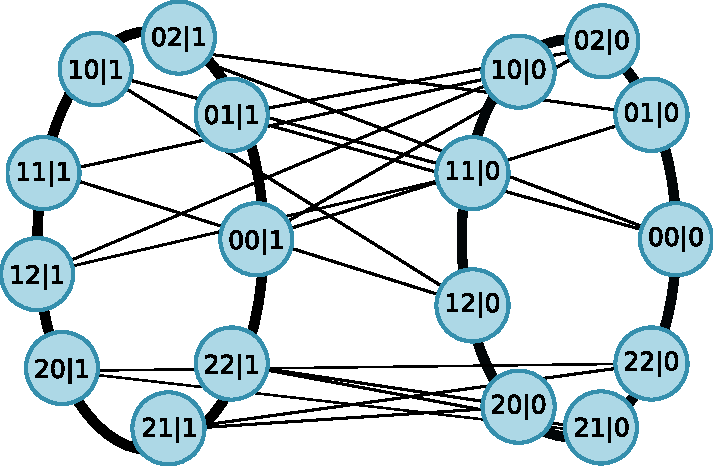
\includegraphics[width=.7\columnwidth]{images/nocycles_proof.pdf}
    \caption{Exclusivity graph for the instrumental scenario $233$, showing the
        impossibility of having cycles with more than $5$ vertices. To simplify the figure cliques are
    represented by bold lines between vertices.}
    \label{fig:2mn_nocycle_proof}
\end{figure}
Any $n$-cycle with at least $5$ vertices must then have at least $3$ mutually
connected vertices belonging to the same $x$, so they can never form a
cycle-graph.
Similarly we can show that there cannot be any induced odd anticycle with $5$ or more
vertices.

\section*{There are no cycles $C_n$ with $n \ge 7$ in the $l22$ instrumental scenario.}
%\label{sec:c5only_proof}
In the following we prove that there cannot be a odd anticycle with more than
$5$ vertices in the exclusivity graph associated to an instrumental scenario of
the type $l22$.

\begin{figure}[h]
    \centering
    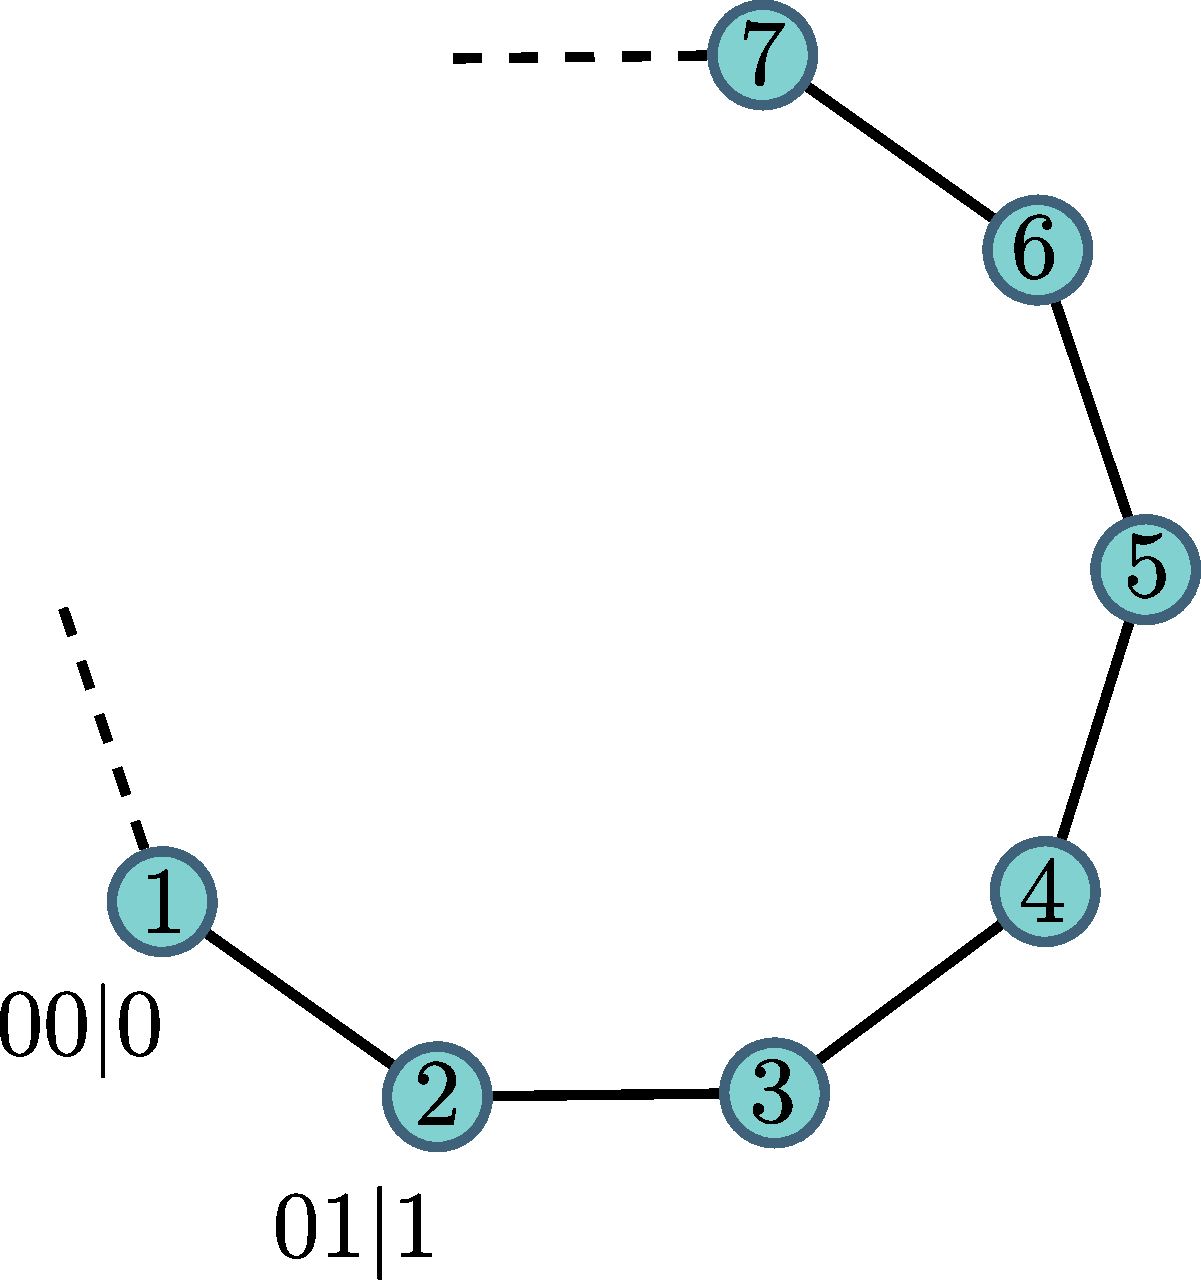
\includegraphics[width=.6\columnwidth]{images/cycle_proof.pdf}
    \caption{Proof of the impossibility of having cycles with $7$ nodes or more
    in the $d22$ scenario.}
    \label{fig:cycle_graph_proof}
\end{figure}

Two different events $ab|x$ and $a'b'|x'$, are exclusive if one of these two conditions is true:
\begin{enumerate}
    \item $x=x'$.\label{en:rule1}
    \item $a=a'$ and $b \neq b'$.\label{en:rule2}
\end{enumerate}
Suppose we have a cycle $C_n$ with $n \ge 7$, as in fig.~\ref{fig:cycle_graph_proof},
and consider that node $2$ in this graph corresponds to an event which we can arbitrarily identify as $00|0$.
Among its neighbors $1$ and $3$, one will necessarily need to satisfy rule
\ref{en:rule2} (they cannot both satisfy rule \ref{en:rule1} or the three nodes
would be a clique.
So without loss of generality we can assign the event $01|1$ to $3$.
Since nodes $5,6,7$ must not satisfy rule \ref{en:rule2} with both $2$ and $3$, then they must have $a = 1$.
Moreover $7$ and $5$ must have the same $b$, different from $6$. In the same way $1$ must not satisfy rule \ref{en:rule2} with $6,5$ and $3$, so it
needs to have $a=0$ and $b=1$. At this point, since we only have values
$\{0,1\}$ for $a$, we cannot avoid node $4$ to be linked to one of the nodes
$1,2,6,7$. Thus, the corresponding graph cannot be a cycle.

\begin{thebibliography}{}
%    \bibitem{pearlbook} J. Pearl, 
%        {\em Causality: models, reasoning, and inference.}
%        Cambridge University Press, (2000).
%    \bibitem{pearl1995} J. Pearl, 
%        {\em On the testability of causal models with latent and instrumental variables}, 
%        Proceedings of the Eleventh conference on Uncertainty in artificial
%        intelligence. Morgan Kaufmann Publishers Inc. (1995).
%    \bibitem{bonet2001} B. Bonet, {\em Instrumentality tests revisited},
%        Proceedings of the Seventeenth conference on Uncertainty in artificial
%        intelligence. Morgan Kaufmann Publishers Inc. (2001).
%            \bibitem{Wooldridge2015} J. M. Wooldridge, {\em Introductory econometrics: A modern approach}. Nelson Education, 2015.
%       \bibitem{Ramsahai2012} R. R. Ramsahai, {\em Causal bounds and observable constraints for non-deterministic models},
%        Journal of Machine Learning Research 13, 829 (2012).
%        \bibitem{Kedagni2017}  D. Kédagni, I. Mourifie, {\em Generalized instrumental inequalities: Testing the IV independence assumption}, available at SSRN (2017).
%    \bibitem{chaves2018} R. Chaves, G. Carvacho, I. Agresti, V. Di Giulio, L. Aolita,
%        S. Giacomini, F. Sciarrino, 
%        {\em Quantum violation of an instrumental test}, 
%        Nature Physics 14.3 291 (2018).
%     \bibitem{himbeeck2018} T. Van Himbeeck, J. B. Brask, S. Pironio, R. Ramanathan, A. B. Sainz, E. Wolfe, 
%        {\em Quantum violations in the Instrumental scenario and their relations to the Bell scenario},
%     \bibitem{cabello2014} A. Cabello, S. Severini, A. Winter,
%         {\em Graph-theoretic approach to quantum correlations}, 
%         Physical review letters, 112, 040401 (2014).
     \bibitem{rabelo2014} R. Rabelo, C. Duarte, A. J.  López-Tarrida, M. T. Cunha, A. Cabello, 
         {\em Multigraph approach to quantum non-locality.}
         Journal of Physics A: Mathematical and Theoretical, 47, 424021 (2014).
%       \bibitem{CHSH}J.F. Clauser; M.A. Horne; A. Shimony; R.A. Holt, {\em Proposed experiment to test local hidden-variable theories}, Phys. Rev. Lett. 23, 880 (1969).
%    \bibitem{economic} P. G. Wright, \emph{The tariff on animal and vegetable oils}, The Macmillan Company, (1928).
%    \bibitem{economic2} C. W. J. Granger, \emph{Investigating causal relations by econometric models and cross-spectral methods}, Econometrica, 424 (1969).
%    \bibitem{economic3} N. Cartwright, \emph{Causal Structures in Econometrics:On the Reliability of Economic Models},Recent Economic Thought Series \textbf{42}, pp 63-89 (1995).
%         \bibitem{Janzing2013} D. Janzing, et al. {\em Quantifying causal influences}, The Annals of Statistics 41, 2324 (2013).
%     \bibitem{bell1964} J. S.Bell, {\em On the Einstein Podolsky Rosen Paradox}, Physics 1, 195 (1964).
%    \bibitem{ried2015} K. Ried, et al. {\em A quantum advantage for inferring causal structure}, Nature Physics 11, 414 (2015).
%     \bibitem{Costa2016}  F. Costa, and S. Shrapnel. {\em Quantum causal modelling}, New Journal of Physics 18, 063032 (2016).
%     \bibitem{Wolfe2016} E. Wolfe, R. W. Spekkens, and T, Fritz. {\em The inflation technique for causal inference with latent variables}, arXiv:1609.00672 (2016). 
%    \bibitem{acin2015} A. Acín, et al. {\em A combinatorial approach to nonlocality and contextuality}, Communications in Mathematical Physics 334, 533 (2015).
%    \bibitem{nielsen_chuang} M. A. Nielsen, Michael \& I. Chuang. 
%    {\em Quantum computation and quantum information.} (2002)
    
%     \bibitem{almostquantum2015} M. Navascués, Y. Guryanova, M. J. Hoban, \& A. Acín, {\em Almost quantum correlations.}
%         Nature Communications 6, (2015).
\bibitem{npa2008} M. Navascués, S. Pironio, \& A Acín, 
         {\em A convergent hierarchy of semidefinite programs characterizing the
         set of quantum correlations.}
         New Journal of Physics 10, 073013 (2008).
%   \bibitem{knuth} D. Knuth, {\em The sandwich theorem}, The Electronic Journal of Combinatorics 1, 1 (1994).
%     \bibitem{lovasz} L. Lovász, 
%         {\em An Algorithmic Theory of Numbers, Graphs, and Convexity.}
%         CBMS Regional Conference Series in Applied Mathematics (1986), §3.2.
% \bibitem{henson2014} J. Henson, R. Lal, M. F. Pusey. {\em Theory-independent limits on correlations from generalized Bayesian networks}, New Journal of Physics 16, 113043 (2014).
%   \bibitem{kcbs2008} A. A. Klyachko, M. A. Can, S. Binicioğlu, A. S. Shumovsky. {\em Simple test for hidden variables in spin-1 systems.}
%         Physical review letters, 101(2), 020403 (2008).
%   \bibitem{cglmp} D. Collins, et al. {\em Bell inequalities for arbitrarily high-dimensional systems}, Physical review letters 88, 040404 (2002).
   
%   \bibitem{spgth} M. Chudnovsky, N. Robertson, P. Seymour, \& R. Thomas, 
%         {\em The strong perfect graph theorem.} 
%         Annals of mathematics, 51-229 (2006).
         
%    \bibitem{carvachoepl} G. Carvacho, R. Chaves, \& F. Sciarrino, 
%        {\em Perspectives on experimental quantum causality.} 
%        EPL (Europhysics Letters), Volume 125, Number 3

     %\bibitem{tomita2006} E. Tomita, A. Tanaka, \& H. Takahashi,
     %    {\em The worst-case time complexity for generating all maximal cliques
     %    and computational experiments.} 
     %    Theoretical Computer Science 363, 28–42 (2006).
         
\end{thebibliography}


\end{document}
